%
%Chapter 6
%
\chapter{First Iteration of Amplifier Testing}
The first version of the test setup and procedure was not well documented or maintained. Due to hardware changes that were too costly to warrant a complete re-fabrication, every amp card had to first be electrically reworked. The post-rework test was a simple continuity and resistance check with a multimeter to make sure all new connections were stable. Amps were then hooked up to a function generator and power supply using jumper wires from their connectors. Input and output were viewed on an oscilloscope to ensure proper amplification. While this was supposed to be a sufficient emulation of their requirements in the system, the entire procedure was loosely documented and not well-enforced enough to ensure long term reproducability and reliability.
\section{Electrical Rework}
One of the first tasks I was given upon entering the group was to help rework each amp. The first issue was that the amplifier power rails (+15V/-5V) were not connected by default. Each amplifier's power rails had to be soldered to the power output using jumper wires. This first step already provided too much room for error, as jumper wires for power distribution would not necessarily be a better choice than simply integrating power lines into the PCB. Adding a person's hand solder in between increased the risks of cold solders or accidental shorts which are completely unacceptable for power pins. \par
\begin{figure}[!htb]
	\includegraphics*[width=15cm]{amp_power_rework}
	\centering
	\caption{Rework of the power rails}
	\centering
	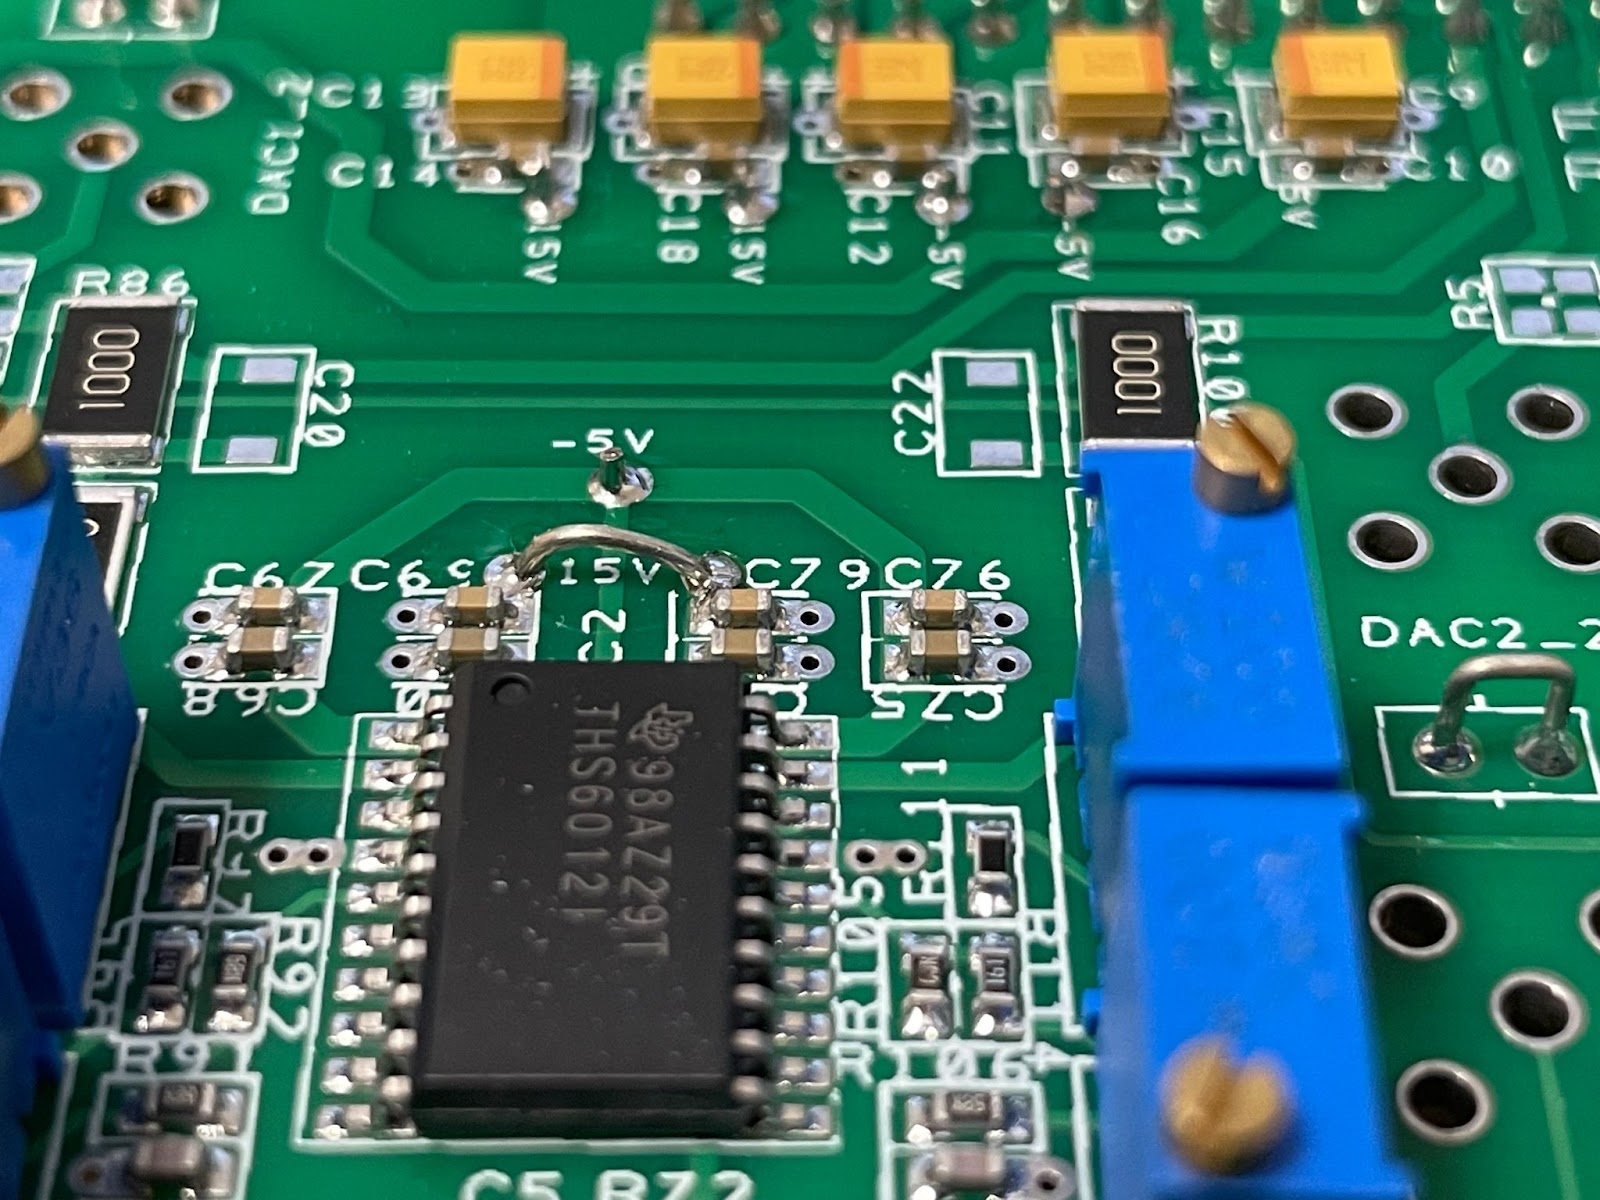
\includegraphics[width=15cm]{reworked_power_rails.jpg}
	\centering
	\caption{Power rails post-rework}
\end{figure}
\section{Component Replacement}
After bridging the power planes on the board, potentiometers and resistors had to be removed and replaced. The potentiometers were initially 100 ohms and used to control gain and offset of the amplified signals. These were replaced with 10 ohm potentiometers which was meant to allow more fine-tuned control over these values. The replaced resistors were also changed to new values to increase signal integrity. Once the rework was completed, it was to be given a brief electrical test (mentioned in the overview) to check the quality of all connections. While the continuity and resistance checks served their purpose, they were not sufficient for fully judging quality of the rework or identifying other issues early. \par
\begin{figure}[!htb]
	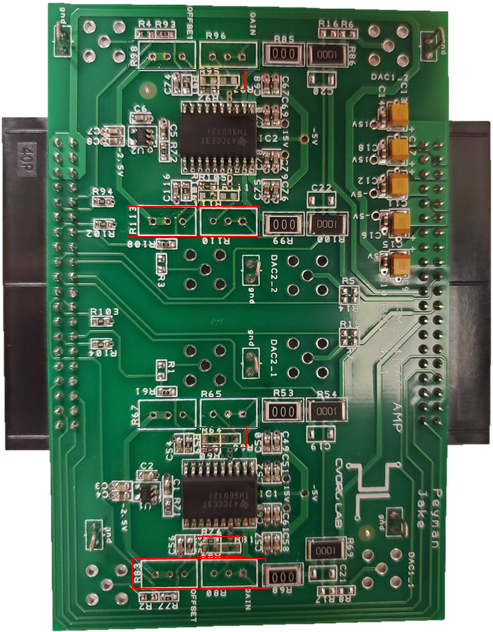
\includegraphics[width=9cm]{amp_components_rework.png}
	\centering
	\caption{Components to be removed and replaced}
	\centering
\end{figure}
The room for human error in this whole process proved to be a massive detriment. Despite a number of group members being experienced solderers, it was impossible to rework such a high volume of boards at a consistently high level of quality. The rework process introduced so many faulty cards that every post-rework card had to be ``quality checked" by a senior group member to make sure the rework was acceptable. As usual, adding another intermediary step decreased the reliability of amps and the pool of boards we had available.
\section{Electrical test}
The first stage of the electrical test consisted of the electrical checks mentioned above. There was no enforced procedure beyond following instructions on a document, and a less experienced group member ran the risk of not fully understanding what they were testing. Without detailed instructions or an intimate knowledge of the purpose of the amp, this electrical check proved to be less and less useful. \par
\begin{figure}[!htb]
	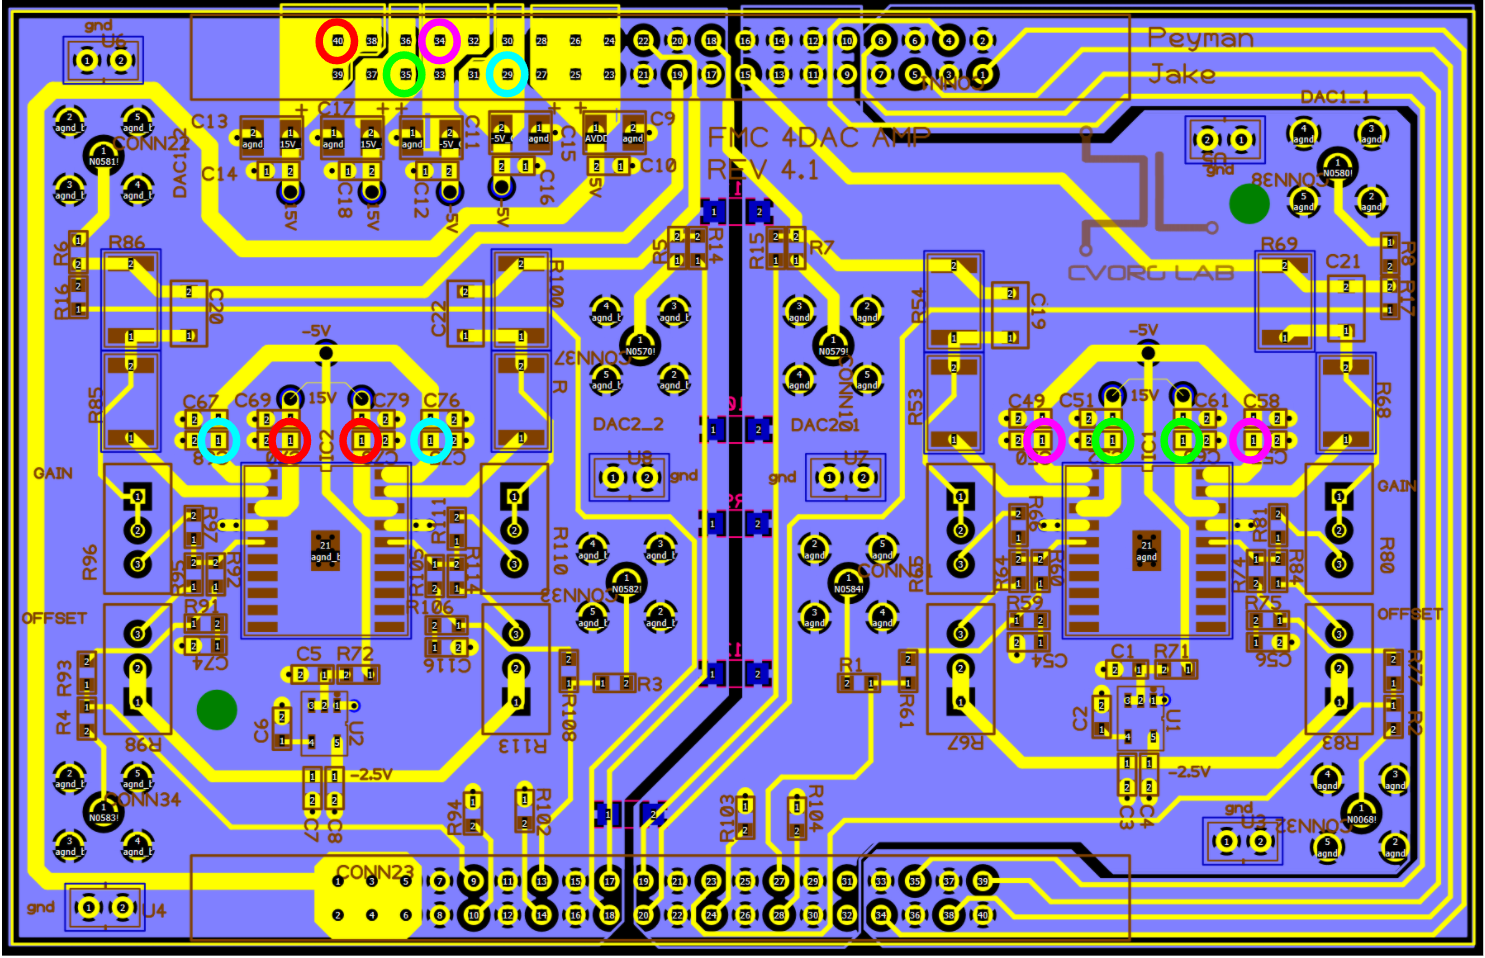
\includegraphics[width=12cm]{amp_rework_continuity.png}
	\centering
	\caption{Official documentation for the continuity checks}
	\centering
\end{figure}
\begin{figure}[!htb]
	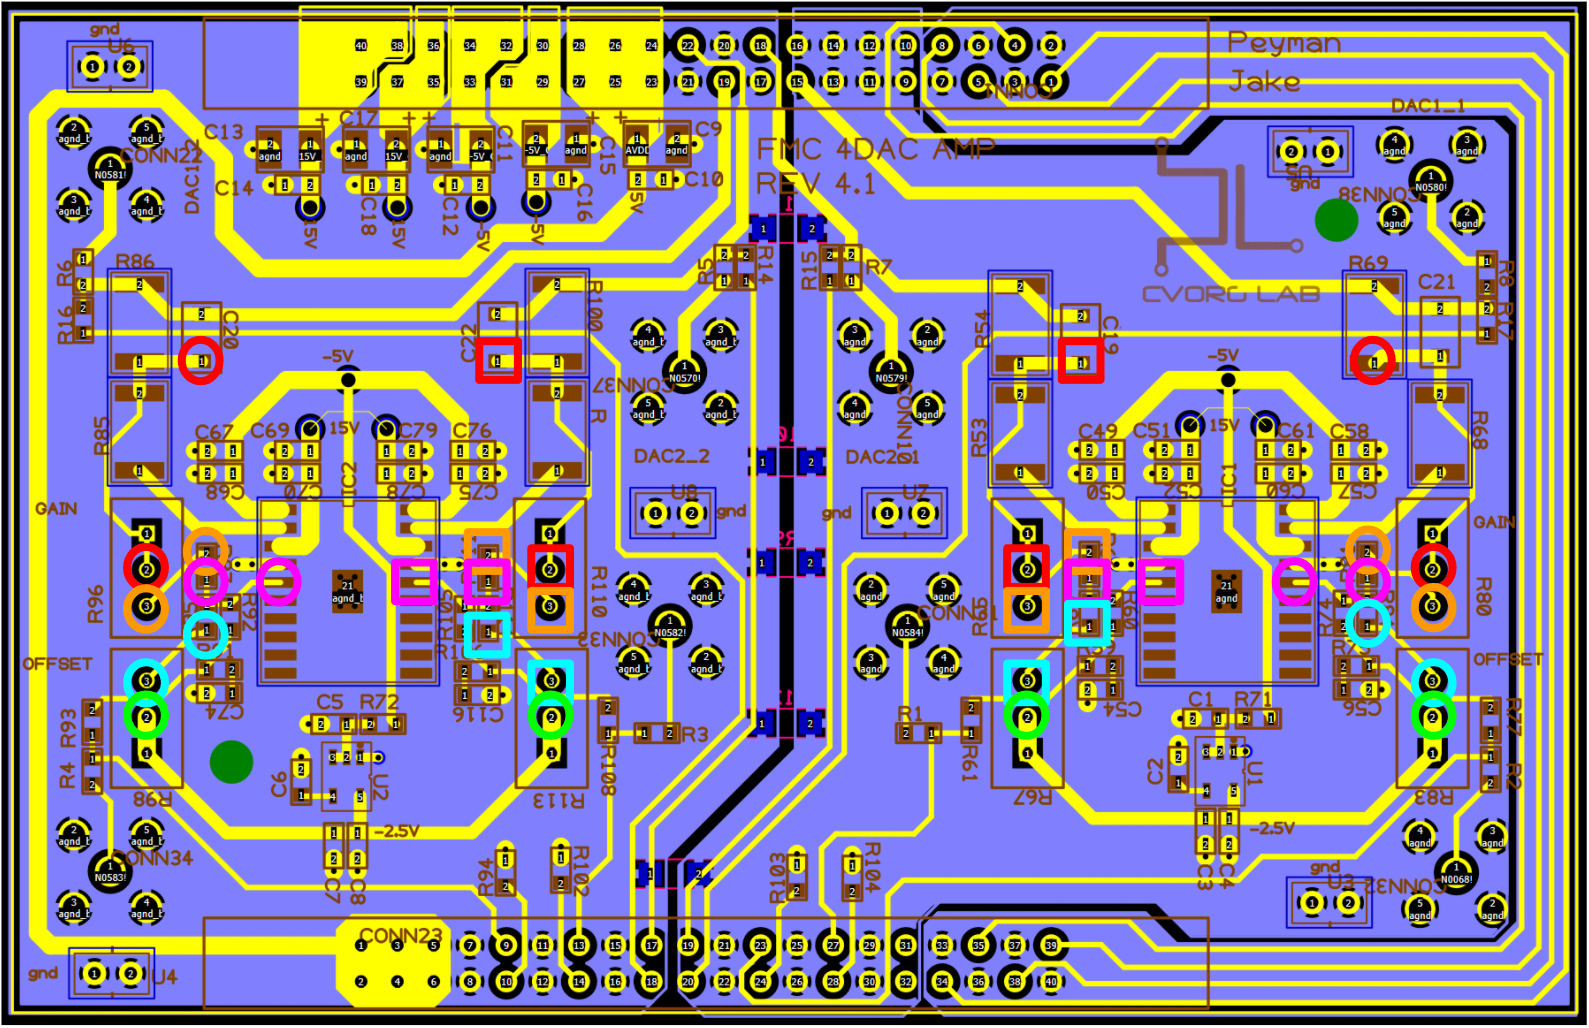
\includegraphics[width=12cm]{amp_rework_test_components.png}
	\centering
	\caption{Official documentation for checking replaced components}
	\centering
\end{figure}
The next testing stage involved hooking up instruments to simulate the type of load the amp card would have to support. This entire part of the procedure was the least well documented or understood and slowed down the validation process quite a bit. Simple breakout boards were hand-soldered for the amp connectors. Inputs were on the bottom connector and plugged into a function generator. Outputs were on the top connector and included pins for power connections (+15/-5) as well as output to the oscilloscope.
\begin{figure}[!htb]
	\centering
	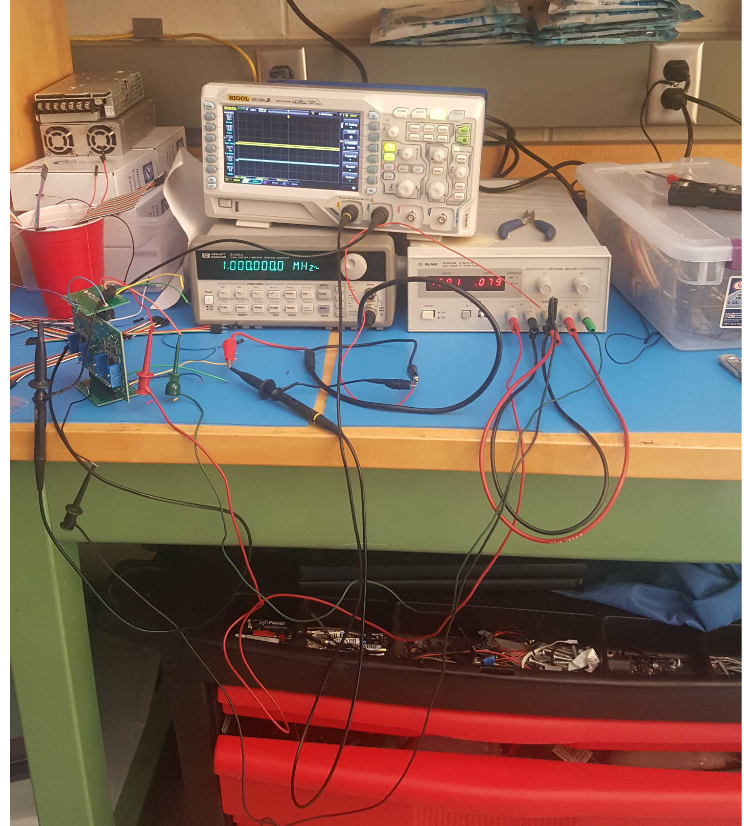
\includegraphics[width=0.5\textwidth]{amp_testing_setup}
	\caption{One of the only official pictures for a completed test setup}
\end{figure}
\subsection{Function generator}
The function generator settings used in the test were rather generic and barely modeled a realistic input for the amps in our system. Input was configured as a 1MHz square wave with an amplitude of 363mV and offset of 318mV. This function was also connected to an oscilliscope to compare against output. Using a high-speed square wave input was definitely a good idea, as a functional amplifier would output an equally square wave. Faulty components would not be able to replicate such sharp rise and settling time. The major downfall of this approach was that the function generator had to be individually tied to each of the card's four input channels, greatly increasing the amount of time a tester had to spend on moving pins and connectors. Having to manually set the wave up was also not the best idea, as this just added another area for the tester to make a mistake.
\begin{figure}[!htb]
	\centering
	\begin{subfigure}[b]{0.43\textwidth}
		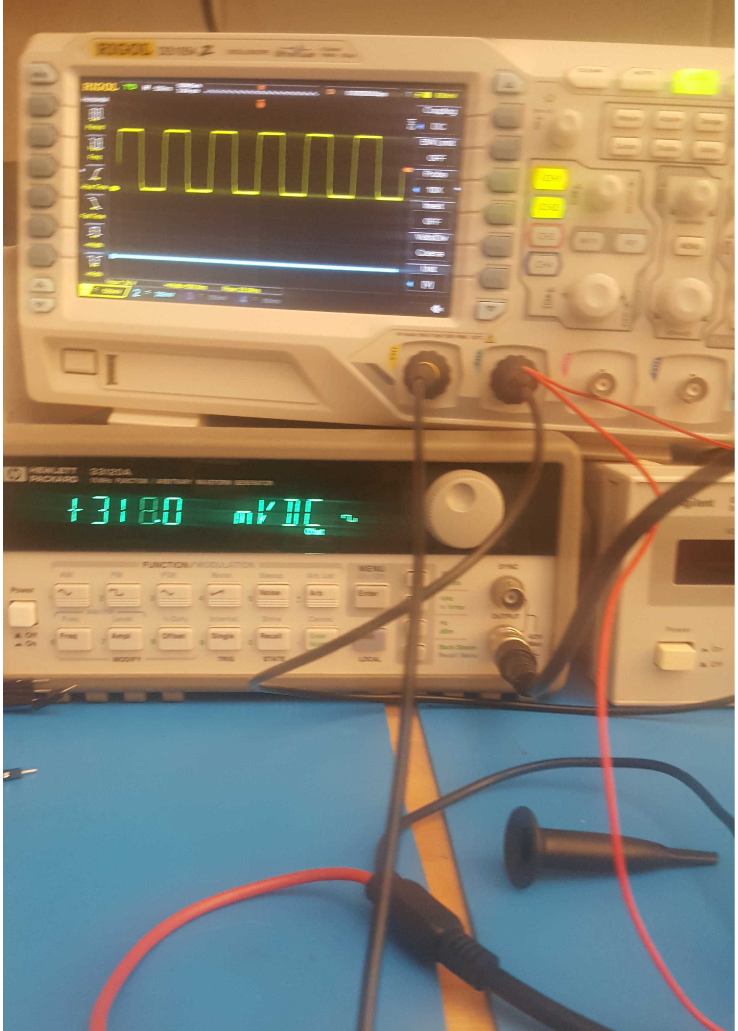
\includegraphics[width=\textwidth]{amp_functiongen_settings}
		\centering
		\caption{Function generator settings}
		\centering
	\end{subfigure}
	\hfill
	\begin{subfigure}[b]{0.5\textwidth}
		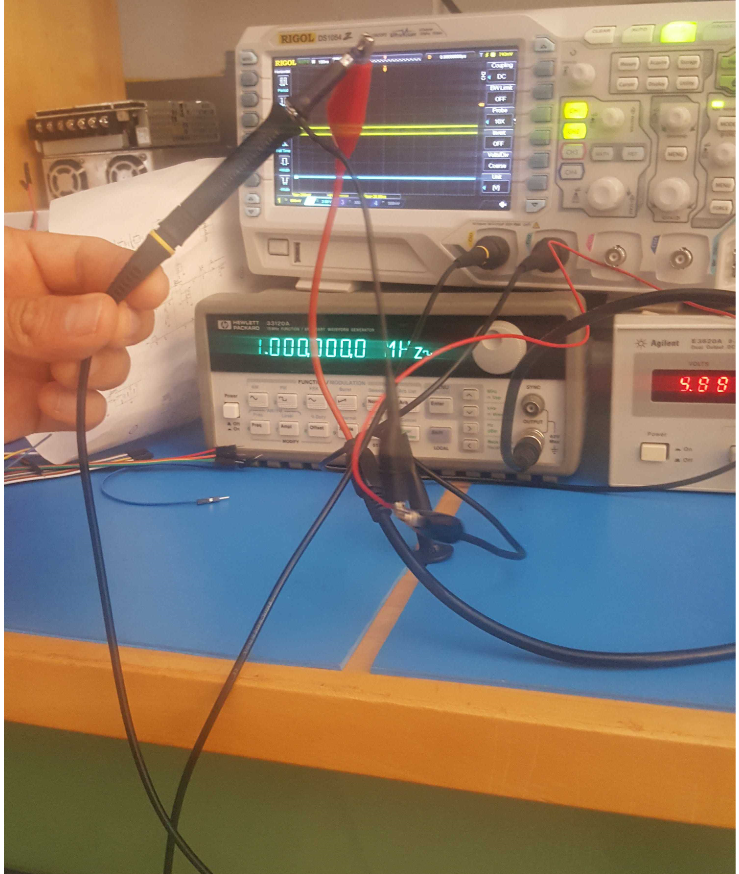
\includegraphics[width=\textwidth]{amp_functiongen_connection}
		\centering
		\caption{Function generator to scope}
		\centering
	\end{subfigure}
	\caption{Offical documentation for setting up the function generator. Insufficient to teach anybody new how to use the equipment.}
\end{figure}
\subsection{Power supply}
Setting up the power rails was a little bit less involved. The user only needed to attach +15V, -5V, and GND to the top breakout board. Connections were still made using extruding jumper wires and alligator clips, yet another point of concern when testing a large number of amps. There were hardly any examples of what a correct setup would look like in the testing document at this point.
\begin{figure}[!htb]
	\centering
	\includegraphics*[width=0.8\textwidth]{amp_powersupply}
	\caption{Official reference image for the amp power supply}
\end{figure}
\subsection{Measuring Output}
As mentioned before, output would be measured on an oscilloscope. Amplitude of input and output could be easily compared by human eyes and the next channel would be connected. This was a slow process that involved manyally re-attaching input and output alligator clips. If gain or offset needed to be tweaked, the tester was to turn their respective potentiometers and observe output. The move to 10 ohm potentiometers greatly decreased their effect on the circuit at all and ended up being more of a nuisance than a useful control signal.
\begin{figure}[!htb]
	\centering
	\includegraphics*[width=0.5\textwidth]{amp_scope_output}
	\caption{Official example of oscilloscope output. Yellow=input, blue=output}
\end{figure}
\section{Lessons Learned}
In conclusion, learning and using the amplifier rework and test procedures was a difficult task that left far too much room for interpretation or error. The amplifiers were crucial to the system's integrity but were not thoroughly tested or maintained. The process was slow, tedious and quite disconnected from the functionality of the system. Poor documentation meant that only a few group members truly understood the purpose and functionality of all steps involved. Swapping cards under test required disconnecting the card from its breakout boards that were already precariously grasped by alligator and probe clips from the instruments. The breakout board pins were not even labled, so it was difficult to determine if issues were due to the user or hardware. This procedure may have filled its need when first conceived, but proved to be unsustainable as the project scaled up. A careful re-examination was required to understand what needed to be tested and what could be improved.
